\documentclass[10pt,a4paper,ngerman]{scrartcl}
\usepackage[utf8]{inputenc}
\usepackage[ngerman]{babel}
\usepackage[T1]{fontenc}
\usepackage{amsmath}
\usepackage{amsfonts}
\usepackage{amssymb}
\usepackage{makeidx}
\usepackage{graphicx}
\usepackage{epstopdf}
\usepackage[onehalfspacing]{setspace}
\usepackage{array}
\usepackage{upgreek}
\usepackage{float}
\usepackage{csquotes}
\usepackage{chemformula}
\usepackage{chemgreek}
\usepackage{chemmacros}
\chemsetup{modules=all}
\usepackage{tikz}
\usepackage{siunitx}
\sisetup{locale = DE,per-mode = symbol}
\usepackage{esvect}
\usepackage{geometry}
\usepackage{pdfpages}
\usepackage[font=small]{caption}
%\usepackage[version=4]{mhchem}
\usepackage[backend=biber, style=chem-angew]{biblatex}
\addbibresource{ROMP.bib}
\usepackage{tabularx, booktabs, multirow}
\usepackage[pdfborder={0 0 0}]{hyperref}
\usepackage{scrlayer-scrpage}%Header für die KOMA-script -Klasse
%\usepackage{hyperref}
\usepackage{pgfplots}
\usepackage{textgreek}


\newcommand{\tildenu}{{\fontencoding{LGR}\selectfont\accperispomeni\textnu}}
\captionsetup{format=plain}
\chemsetup[phases]{pos=sub}
\chemsetup[redox]{pos=top}
\chemsetup[redox]{align=center}
%\chemsetup[redox]{explicit-sign=true}
%\chemsetup[redox]{roman=false}
\newcommand{\celsius}{^{\circ}\mathrm{C}}
\parindent0pt
\sloppy
\DeclareChemPhase{\s}{s}
\DeclareChemPhase{\l}{l}
\DeclareChemPhase{\g}{g}
\renewcaptionname{ngerman}{\figurename}{Abb.}
\renewcaptionname{ngerman}{\tablename}{Tab.}
\geometry{bottom=100pt} \geometry{top=80pt}
\newcommand{\m}{\mathrm{m}}
\newcommand{\K}{\mathrm{K}}
\newcommand{\J}{\mathrm{J}}
\newcommand{\gr}{\mathrm{g}}
\newcommand{\kg}{\mathrm{kg}}
\newcommand{\mol}{\mathrm{mol}}
\newcommand{\Pa}{\mathrm{Pa}}
\newcommand{\ad}{\mathrm{ad}}
\newcommand{\de}{\mathrm{de}}
\newcommand{\gmol}{\mathrm{\frac{g}{mol}}}
\newcommand{\JKmol}{\mathrm{\frac{J}{K \cdot mol}}}
\newcommand{\kgmss}{\mathrm{\frac{kg}{m \cdot s^2}}}
\newcommand{\loge}{\mathrm{ln}}


\begin{document}
\begin{titlepage}
	\vspace*{2,5cm}
	\begin{center}
		\begin{LARGE}
			\textbf{Polymer Chemie}\\
			\textbf{Ring opening Methathesis Polymerization (ROMP)}\\
		\end{LARGE}
		\vspace{1cm}
		\textbf{Universität Stuttgart}\\
		\vspace*{1,5cm}
		\begin{tabular}{lp{7,5cm}l}
			Author 1:     &Laurens Viehoff\\
            Author 2:     &Felix Roth\\   
			E-Mail 1:      &st183688@stud.uni-stuttgart.de\\
            E-Mail 2:      &st188157@stud.uni-stuttgart.de  \\
			Student-ID 1: & 3676761   \\ 
            Student-ID 2: & 3711192 \\ \\
			Assistentin:  & Patrick Probst  \\ \\ 
		\end{tabular}
		
		\vspace{2cm}
		Version 2\\
	\end{center}

    
\end{titlepage}
\thispagestyle{empty}
\renewcommand{\thepage}{\arabic{page}}
\newpage
\tableofcontents
\setcounter{page}{1}
\renewcommand{\thepage}{\arabic{page}}
\newpage


\section{Theorie}

	\subsection{Koordinative Polyinsertionen}

		Eine der Bekanntesten Polyinsertionen ist die Ziegler-Natta-Reaktion.
		Dabei werden Katalysatoren verwendet, welche ein Element der Gruppen 1-3 mit einem Übergangsmetall der Gruppen 4-8 gebunden haben.
		Beispiele hierfür wären Metallhydride oder Arylidenverbindungen. 
		Im Falle der Ziegler-Natta besteht der Katalysator aus \ch{TiCl4} mit \ch{Et3Al}.
		Die koordinative Polyinsertionen lassen sich in eine Monometallische und eine Bimetallische Polymerisation unterteilen.
		Beide machen sich jedoch die Koordinationseigenschaften des Übergangsmetalls zu nutze.
		So koordiniert eine Doppelbindung an einen freie Stelle des Metalls. 
		Dabei bildet sich mit einem Rest an einer anliegenden Stelle ein viergliedriger Übergangszustand.
		Anschließend klappen die Bindungen so um, dass der Rest an die eine Seite der Doppelbindung übertragen wird.
		Die Kette ist somit um den Rest des Olefins gewachsen.

			\begin{figure}[H]
				\centering
				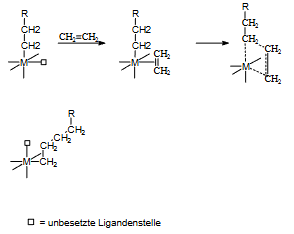
\includegraphics[scale = 1]{Bilder/Monometall.png}
				\caption{Die Abbildung zeigt den Verlauf der monometallischen Polyinsertion. \cite{polyskript}}
				\label{Monometall}
			\end{figure}

		Wichtig hierbei ist, dass der Metallkomplex nicht an der Wachstumsreaktion beteiligt ist und lediglich
		das neue Monomer an das Polymer koordiniert.\\
		Die Reaktion kann auf drei unterschiedliche Weisen abgebrochen werden.
		So kann die Reaktion durch eine $\beta$-H-Eliminierung abgebrochen werden, 
		oder durch eine Übertragung auf das Monomer. Bei letzterem besteht die Möglichkeit einer Molekulargewichtsregelung durch \ch{H2}.\\

		Beim Bimetallischen hingegen sind, wie der Name bereits sagt, zwei Metallatome beteiligt.
		Dabei wechselwirken die $\pi$-Elektronen des Olefins mit den Orbitalen des Übergangsmetalls.
		Wichtig ist, dass dabei selbst nach der Koordination des Olefins an das Metall keine freie drehbarkeit zwischen der C-C-Bindung möglich ist.
		Genauso beeinträchtigt bleibt die freie drehbarkeit zwischen der Metall-Kohlenstoff-Bindung.
		Dies spielt eine große Rolle, da dadurch der Rest, welcher am Olefin gebunden ist, seine relative Position in Richtung der Methylgruppe behält.
		Anschließend bildet sich ein Ring wodurch der Elektronenüberlapp eine neue $\sigma$-Bindung zwischen C(1) und C(3) gebildet wird. 
		Dabei wird die Al-C(3)-Bindung gekappt und es kann sich der Ausgangskomplex mit dem neu hinzugefügten Rest bilden.

			\begin{figure}[H]
				\centering
				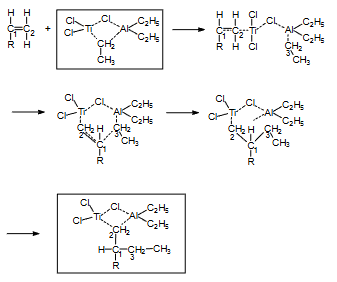
\includegraphics[scale = 1]{Bilder/Bimetallisch.png}
				\caption{Die Abbildung zeigt der Ablauf der bimetallischen Polyinsertion. \cite{polyskript} }
				\label{Bimetallisch}
			\end{figure}
		
		Meist wird bei der Verwendung dieser Mechanismen Monomere wie Propen oder Styrol verwendet,
		durch welche unterschiedliche stereoreguläre Polymerketten gebildet werden können.
		Dabei wird zwischen isotaktisch (in Abb. \ref{taktizitaet} mitte), syndiotaktisch (in Abb. \ref{taktizitaet} rechts) und in ataktisch (in Abb. \ref{taktizitaet} links) unterschieden.
		Bei ersterem zeigen die Reste immer in die selbe Richtung es etsteht die Konfiguration (R,R,R,R,R). 
		Bei einem syndiotaktischen Polymer hingegen sind diese alternierend, es ergibt sich die Konfiguration (R,S,R,S,R,S). 
		Bei letzeren ist die Abfolge komplett zufällig.
		Diese Taktizität hat einen großen Einfluss auf die Eigenschaften des Polymers. 
		Damit ändert sich Beispielsweise der Aufbau der Kristallstruktur,  
		welche wiederum die Eigenschaften des Polymers bestimmen. Weitere Eigenschaften sind die Härte, Sprödigkeit, Formbeständigkeit und der Schmelzpunkt.

		
			\begin{figure}[H]
				\centering
				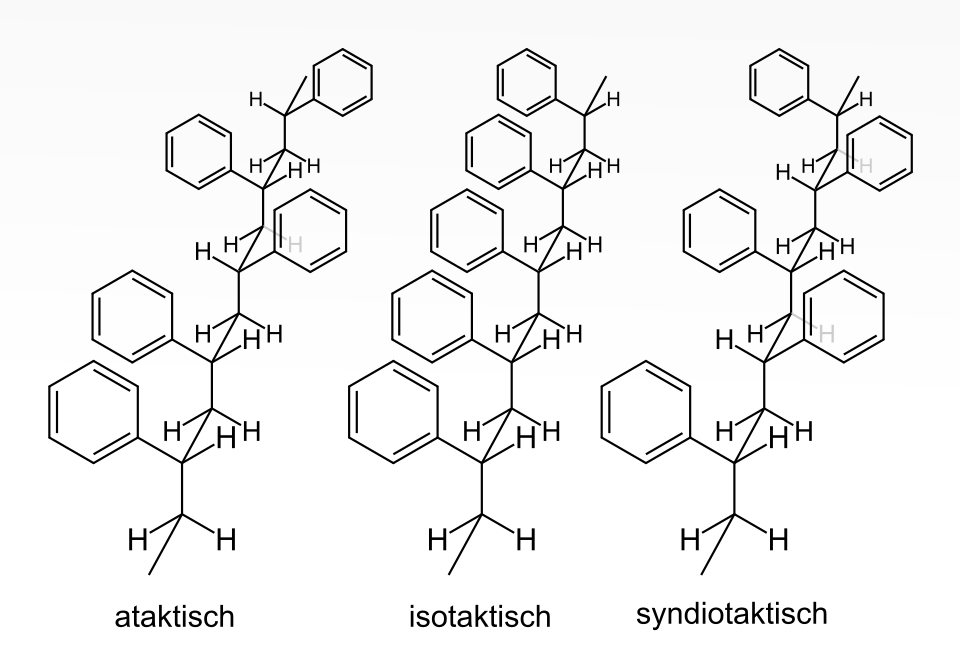
\includegraphics[scale = 0.25]{Bilder/taktizität.png}
				\caption{Die Abbildung zeigt die jeweiligen Taktizitäten welche möglich sind. \cite{noauthor_taktizitat_2025}}
				\label{taktizitaet}
			\end{figure}
		
		
	\subsection{Ring öffnende Methathespolymerisation}

		Die Ring öffnende Methathesenpolymerisation (ROMP) läuft im Allgemeinen nach dem Mechanismus der Olefinmethathese ab.
		Bei diesem findet ein Austausch von Alkenylgruppen zweier Olefine statt. 
		Dies läuft in Gegenwart eines Organo-Metallischen-Katalysators.
		Im Allgemeinen reagieren die beiden Olefine in einer [2+2] Zykloaddition.
		Das dadurch entstandene Metallcyclobutan-Intermediat kann wiederum in einer [2+2] Zykloreversion das Produkt bilden.
		Das Metall wird dabei selbst als Metallalkyliden abgespalten.
		Der große Vorteil dieser Reaktionen ist, dass jeder Schritt im großen und ganzen reversibel ist.
		Ein Nachteil welcher diese Reversibilität mit sich bringt ist, dass eine große Kontrolle über die Triebkraft notwendig sein muss.

			\begin{figure}[H]
				\centering
				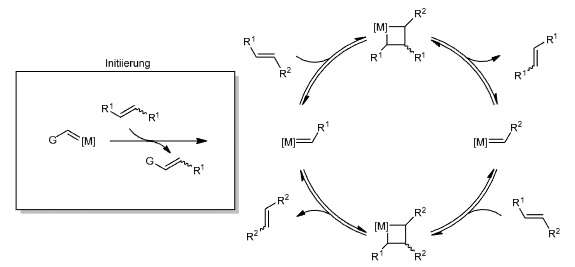
\includegraphics[scale = 0.75]{Bilder/Methathesezyklus.png}
				\caption{Die Abbildung zeigt den Methathesezyklus mit seinen einzelnen Teilschritten. \cite{polyskript}}
				\label{Methathesezyklus}
			\end{figure}

		In unserem Fall wird der Grubbs-Katalysator der ersten Generation verwendet welcher auch in Abb. \ref{Grubbs} zu sehen ist.
		Im Allgemeinen ist es wichtig zu wissen, dass es viele unterschiedliche Katalysatoren für unterschiedliche Gebiete mit unterschiedlichem Nutzen gibt.
		
			\begin{figure}[H]
				\centering
				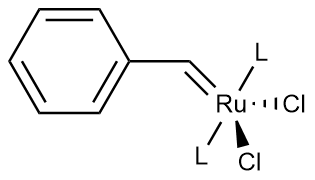
\includegraphics[scale = 0.5]{Bilder/Grubbs.png}
				\caption{Die Abbildung zeigt den Grubbs-I-Katalysator.}
				\label{Grubbs}
			\end{figure}

		Im Falle der ROMP wird diese Methathese mittels eines bizyklischen Olefins durchgeführt, welcher im Laufe des Kettenwachstums geöffnet wird.
		Die wie bereits oben genannte Triebkrafft, liegt hierbei in der Ringspannung welche durch das Öffnen verloren geht.
		Der allgemeine Ablauf der ROMP ist in Abb. \ref{ROMP} gezeigt.

			\begin{figure}[H]
				\centering
				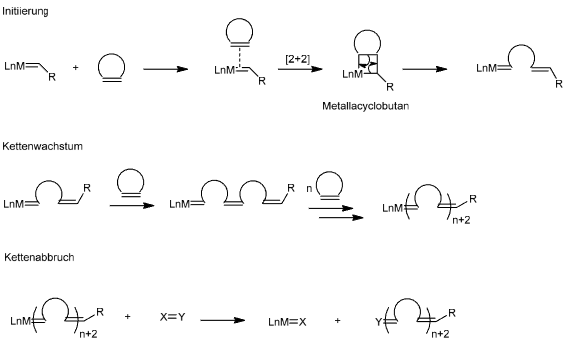
\includegraphics[scale = 0.75]{Bilder/ROMP.png}
				\caption{Die Abbildung zeigt den Ablauf der Ringöffnenden Methathesenpolymerisation. \cite{polyskript}}
				\label{ROMP}
			\end{figure}

\section{Durchführung}

	In allen Versuchsteilen sollte unter Schlenk-Bedingungen gearbeitet werden.
	Jedoch wurde im ersten Versuchsteil nach absprache mit dem Assistenten zwar angeschlenkt, es wurde jedoch nicht ausgeheitzt, 
	da dies ausprobiert werden sollte und es theoretisch keinen Unterschied machen sollte.

	\subsection{Polyinsertion}

		In einem Kolben mit Septum wurde Heptan (\SI{25}{ml} aus der SPS) vorgelegt.
		Es wurde eine Spritze mit \ch{TiCl4} (\SI{0.5}{ml}, 4.17 mmol, 0,04 Äq) zugegeben. 
		Anschließend sollte Triisobutylaluminium-Lösung (\SI{12,5}{ml}, 25\% in Hexan) im Zeitraum von 20 min zugegeben werden.
		Dieser Schritt wurde jedoch falsch gemacht und es wurde alles schnell zugegen.
		Der Kolben wurde während des Zugebens mit einem Wasserbad gekühlt.
		Nach 10 min wurde Styrol (\SI{12.5}{ml}, 104,22 mmol, 1 Äq) auf einmal zugegeben und bei 74°C für 2-3h geheitzt.
		Anschließend wird auf Raumtemperatur abgekühlt und die Reaktion wird mit in Methanol gelöstem \ch{HCl} (\SI{100}{ml}) abgebrochen.
		Das Polymer wurde in Methanol gewaschen und abfiltriert.
		Das Produkt wurde im Vakuumtrockenschrank bei 60°C getrocknet.
		
	\subsection{ROMP}

		In einem Schlenkkolben wurde trockenes DCM (\SI{20}{ml}) vorgelegt. 
		Es wurde Monomer (\SI{1.00}{g}, \SI{3,29}{mmol}, 1 Äq) eingewogen und in den Kolben gegeben.
		Der Katalysator (\SI{43}{mg}, 1mol\%) wurden in ein Schnappdeckelglas eingewogen und in trockenem
		DCM (\SI{2}{ml}) gelöst.
		Die Lösung wurde anschließend in einem Schuss zugegeben und die Lösung wurde für eine Stunde bei Raumtemperatur gerührt.
		Nach einer Stunde wurde eine Pipette \SI{2}{ml} entnommen und in Methanol gegeben.
		Zur restlichen Lösung wurden \SI{20}{ml} Ethylvinylether zugegeben und weitere 10 Minuten gerührt.
		Anschließend wird auch hier das Polymer in Methanol gefällt abfiltriert und getrocknet.

\section{Auswertung}

	Der erste Versuchsteil hat nicht gut funktioniert, da beim Zugeben der Aluminiumalkyl Lösung alles auf einmal zugegeben wurde.
	Dies hatte eine Lösung mit schwarzem Feststoff zufolge.
	Das Produkt konnte deshalb nicht sauber isoliert werden, weshalb der Versuch als felgeschlagen gewertet wurde und keine Ausbeute bestimmt werden konnte.\\
	Der zweite Versuchsteil wurde gemäß der Vorschrift durchgeführt. 
	Nach Wiegen konnte eine Ausbeute von 11,6\% nach folgender Rechnung erhalten werden.

			\begin{eqnarray}
				 \text{Ausbeute} =& \frac{m_\text{Produkt}}{m_\text{Edukt}} \cdot 100\%\\
				 =& \frac{\SI{0.116}{g}}{1} \cdot 100\% \\
				 =& 11,6\%
			\end{eqnarray}

\section{Fragen}

	\subsection{Polyinsertion}

		\subsubsection{Frage 1}

			Die Extraktion mit Methylethylketon und Toluol sorgt für eine Auftrennung des Produkts, welches möglicherweise aus Polymer und davon eingeschlossenem Titan- 
			und Aluminiumalkylen besteht. Somit wird im Ganzen das Polymer sauberer. 
			Unteranderem haben isotaktische und ataktische Polymere unterschiedliche Löslichkeiten, welche zur Trennung ausgenutzt werden können.  

		\subsubsection{Frage 2}

			Verwendet wurden bei der Reaktion \SI{0,5}{ml} $\ch{TiCl4}$ und \SI{12,5}{ml} Styrol. Mit den entsprechenden Dichten und molaren Massen, entspricht das einem 
			Verhältnis von (Ti:Styrol= 0,4:10,9), welches auch mit folgender Gleichung hergeleitet werden kann.

			\begin{equation}
				\frac{n_\text{Ti}}{n_\text{Styrol}} = \frac{\frac{\rho_\text{Ti} \cdot V_\text{Ti}}{M_\text{Ti}}}{\frac{\rho_\text{Styrol} \cdot V_\text{Styrol}}{M_\text{Styrol}}} = \frac{\frac{\SI{1,728}{\frac{g}{ml}} \cdot \SI{0,5}{ml}}{\SI{189,71}{\frac{g}{mol}}}}{\frac{{\SI{0,91}{\frac{g}{ml}} \cdot \SI{12,5}{ml}}}{\SI{104,15}{\frac{g}{mol}}}} = 0,0417 \text{.}
			\end{equation}

			Die Stoffmengenkonzentration des Katalysators entspricht dabei der Stoffmengenkonzentration des $\ch{TiCl4}$ für das ganze Volumen und somit

			\begin{equation*}
				M_\text{\ch{TiCl4}} = \frac{\frac{\rho_\text{Ti} \cdot V_\text{Ti}}{M_\text{Ti}}}{V_\text{ges}} = \frac{\frac{\SI{1,728}{\frac{g}{ml}} \cdot \SI{0,5}{ml}}{\SI{189,71}{\frac{g}{mol}}}}{\SI{25}{ml} + \SI{0,5}{ml} + \SI{12,5}{ml} + \SI{12,5}{ml}} = \SI{90,185}{\frac{mmol}{l}} \text{.}
			\end{equation*}

		\subsubsection{Frage 3}

			Die nachfolgende Abbildung zeigt die Fischer- und die Natta-Projektion auf.

			\begin{figure}[H]
				\centering
				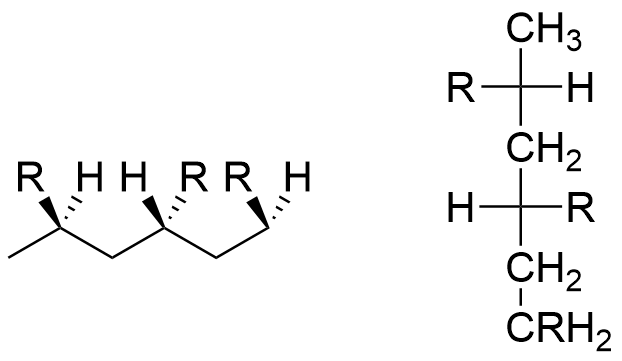
\includegraphics[scale = 0.4]{Bilder/Natte-Fischer-Projektion.png}
				\caption{Abgebildet ist links die Natta- und rechts die Fischer-Projektion des selben hypothetischen Oligomeren.}
				\label{NattaFischerProjektionabb}
			\end{figure}

			Bei der Natta-Prjektion wird die Orientierung der Substituenten durch Keile oder Striche gekennzeichnet, während bei der Fischer Projektion die fortführende 
			Kette immer nach oben und unten geschrieben wird und die Substituenten rechts und links abgehen. Dabei wird auf das Substitutionstetraeder so draufgeschaut, dass 
			die fortführende Kette nach hinten zeigt und vorne die Substituenten stehen. Nach links zeigen dann die Substituenten, welche in der Natta-Projektion nach vorne 
			stehen und umgekehrt.

		\subsubsection{Frage 5}

			Bei LDPE und HDPE ist die Dichte der Hauptunterschied, was dadurch Zustande kommt, dass die Polymerketten bei LDPE nur amorphe Strukturen bilden und HDPE 
			teilkristallin ist. Unteranderem ist HDPE Dichter, da es mehr Verzweigungen aufweist und mehr quervernetzt ist.


		\subsubsection{Frage 6}

			Durch den Sauerstoff in der Etherbindung, würde dieser im bimetallischen Mechanismus zum Titan koordinieren und diesen so desaktivieren.

		\subsubsection{Frage 7}

			HDPE besteht aus teilkristallinen Strukturen aus linearem Polyethylen. Bei LDPE ist die Struktur amorph, da die Ketten zusätzlich verzweigt sind. LLDPE ist 
			ebenfalls amorph, allerdings sind die Verzweigungen weniger lang als bei LDPE, wodurch die Dichte etwas ansteigt. Diese und weitere Strukturen sind nochmal in 
			Abbildung \ref{ROMPstrukturen} aufgeführt.

			\begin{figure}[H]
				\centering
				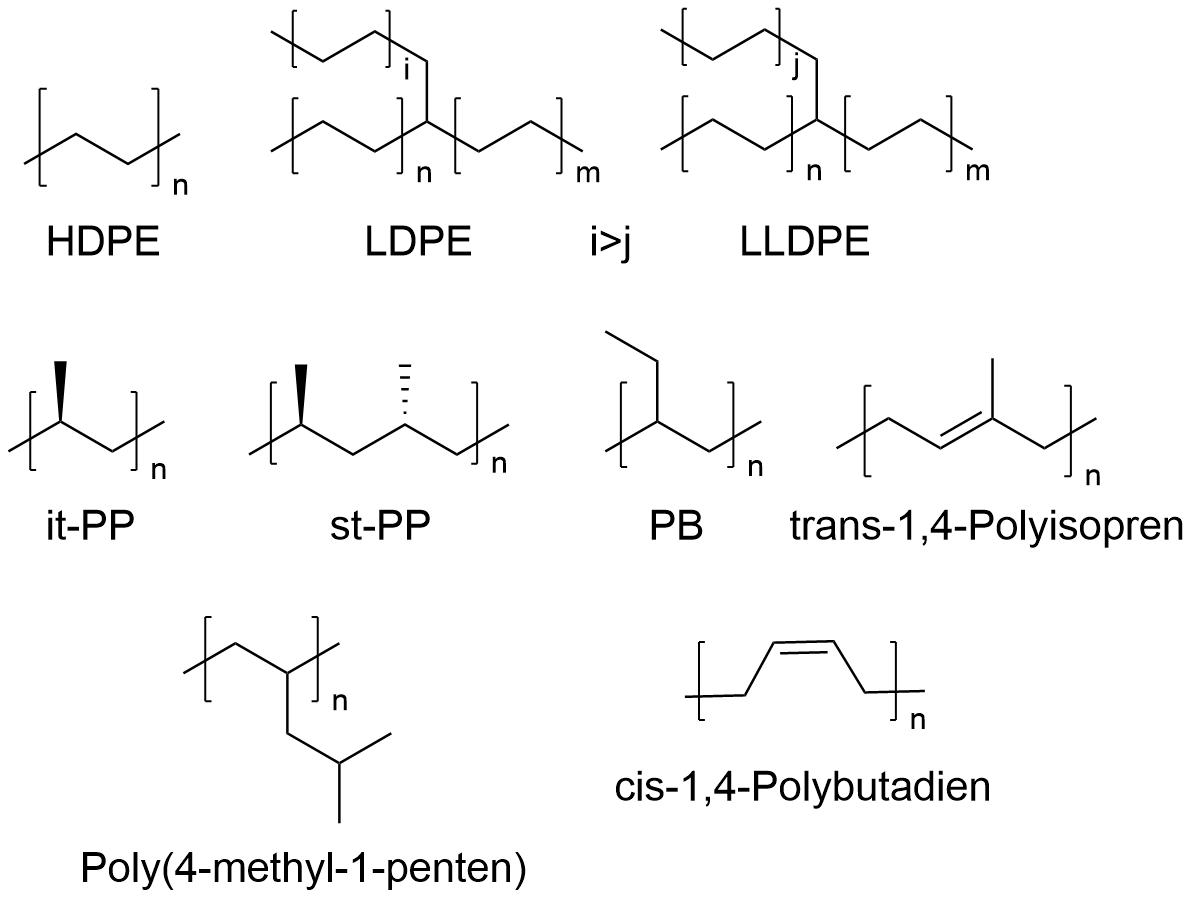
\includegraphics[scale = 0.3]{Bilder/StrukturenROMP.png}
				\caption{Abgebildet sind die Strukturen der Polymere.}
				\label{ROMPstrukturen}
			\end{figure}


	\subsection{ROMP}

		\subsubsection{Frage 1}

			Beim ersten Fällen, bildete sich ein roter Polymerklumpen, der beim zweiten Fällen nicht beobachtet wurde. Das liegt daran, dass beim ersten Fällen noch der 
			Grubbs-Katalysator die Endgruppe bildete und beim zweiten Fällen zuvor entfernt wurde.

		\subsubsection{Frage 2}

			Ethylvinylether bricht die Reaktion ab und ersetzt die Endgruppe. Dabei wird nämlich der Ruthenium-Katalysator gegen ein Kohlenstoff substituiert. Die Reaktion ist 
			anschließend aufgeführt. 

			\begin{figure}[H]
				\centering
				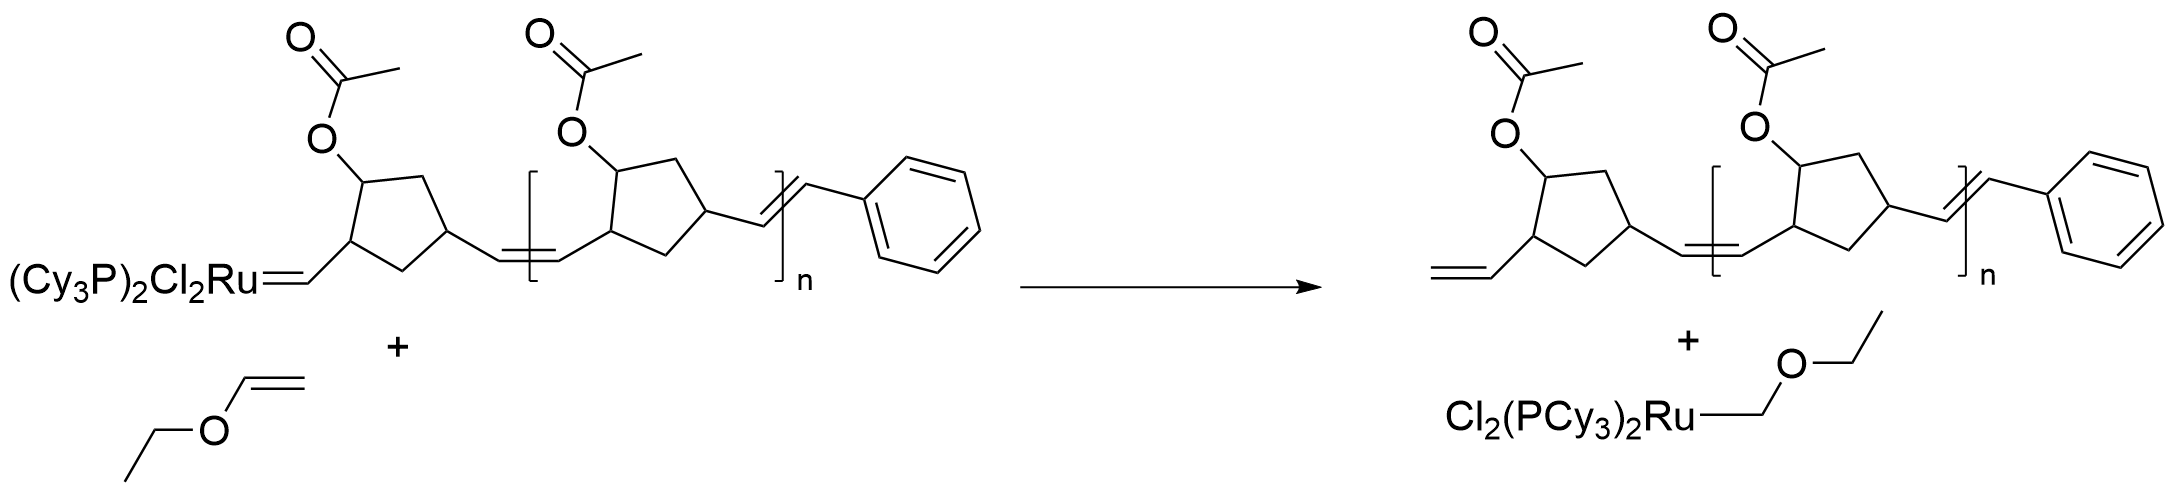
\includegraphics[width = \textwidth]{Bilder/ROMPabbruchethylvinylether.png}
				\caption{Reaktionsgleichung des Abbruchreaktion zwischen dem Grubbs-Polymer und Ethylvinylether.}
				\label{ROMPethylvinyletherabbruch}
			\end{figure}

			Der Grund für die Wahl von Ethylvinylether ist die definierte Endgruppe. Denn bei der Koordinierung von Ethylvinylether an Ruthenium, koordiniert dieses immer 
			nach der Weise aus Reaktion \ref{ROMPethylvinyletherabbruch}. Mit 1-Penten wäre die Endgruppe nicht bekannt und wäre statistisch Verteilt.

		\subsubsection{Frage 3}

			Der Katalysator muss bei der Reaktion so schnell wie möglich hinzugegeben werden, um die Polydispersität möglichst eng zu halten und alle Polymere gleichzeitig 
			starten zu lassen. Die gleiche Begründung lässt sich bei der Durchmischung auch anwenden, je besser durchmischt ist, desto mehr ist das Monomer verteilt und die Ketten werden gleichzeitig gestartet.
			Eine zu hohe Starttemperatur hat ein langsameres Wachstum zur Folge da die meisten Polymerisationen exotherm sind und somit zugefügte Energie gegen die Reaktionskinetik wirkt.
			Durch eine zu hohe Konzentration wird die Reaktion unkontrolliert, da sich die Konzentration direkt auf die Reaktionsgeschwindigkeit auswirkt. 

		\subsubsection{Frage 4}

			Das theoretische Molekulargewicht wird über die Monomermasse und die Katalysatorstoffmenge bestimmt. 
			Damit ergibt sich eine molekulare Masse von

			\begin{equation*}
				M_\text{theo} = \frac{m_\text{Mono}}{n_\text{kat}} = \frac{\SI{1}{g}}{\SI{0,052}{mmol}} = \SI{19230,77}{\frac{g}{mol}} \text{.}
			\end{equation*}

			Die GPC-Messung führte zu einem zahlenmittleren Molekulargewicht von $M_\text{n} = \SI{31000}{\frac{g}{mol}}$ und einem PDI von 1,6. 
			Das bedeutet, dass der eingesetzte Katalysator fast vollständig eine Polymerisation initiiert hat und nur kleine Mengen durch 
			Verunreinigungen desaktiviert wurden. Der PDI zeigt hingegen, dass die Molmassenverteilung relativ eng Verteilt ist und die Ketten nicht 
			sonderlich weit von dem zahlenmittleren Molekulargewicht abweichen.

		\subsubsection{Frage 5}

			Den Katalysator kann nach der desaktivierung mit Ethylvinylether nicht erneut verwendet werden, da der Rest zu inreaktiv ist. Allerdings kann der Katalysator 
			chemisch regeneriert werden, indem der Rest substituiert wird. 

		\subsubsection{Frage 6}

			Um das Polymer löslicher zu gestallten, müssen die Seitenketten variiert werden. Mit Phenylresten wäre das Polymer möglich in Toluol zu lösen, mit ionischen 
			Seitenketten wäre es möglich es in Wasser zu lösen. Die Faktoren die eine Rolle spielen sind Polarität und Bildung guter intermolekularer Wechselwirkungen.
			Wenn jedoch weniger Monomer bei gleichem Katalysator verwendet wird, gibt es keine große Änderung, da nur eine gewisse Anzahl an Monomer verwendet werden kann.
			Das Monomer ist der limitierende Faktor in der Reaktion. 

		\subsubsection{Frage 7}

			Die Wahl des Katalysators kann die Reaktionsgeschwindigkeit verändern. Bei der koordinierung der Monomere an den Ruthenium-Kern muss dieser einen Substituenten 
			abspalten um das Monomer zu koordinieren. Die Wahl dieses Substituenten ist dabei dann Geschwindigkeitsbestimmend. Ist die Dativbindung zwischen dem Liganden und 
			dem Ruthenium-Kern beispielsweise stärker, ist die Reaktion verlangsamt. Ist aber die Bindung schwächer, ist die Reaktion schneller.
			Jedoch kann es teilweise vorkommen, dass für manche Reaktionen ein spezieller Katalysator benötigt wird welcher jedoch teurer ist oder empfindlicher ist.
		
		\subsubsection{Frage 8}

			Der Ausgangskatalysator besitzt ein Carben, welches im singulett oder triplett Zustand vorliegen kann. Je nach dem wäre dieses Signal hochfeld Verschoben. Des 
			weiteren ist die propagierede Spezies ein Cyclobutanderivat, bei welchem nur einfach Bindungen vorliegen und die chemische Umgebung unterschiedlich ist. 
			Dementsprechend wäre dieses Signal wieder verschoben und von dem Signal des Ausgangskatalysators verschieden.

		\subsubsection{Frage 9}

		%Hier schwafelst du was vom NMR, sollten 8 alifatische sein wovon 4, 2, 2 gleich sind und 2 gleiche olefinische, kann aber auch schwer sein, weil E/Z möglich ist

				\begin{figure}[H]
					\centering
					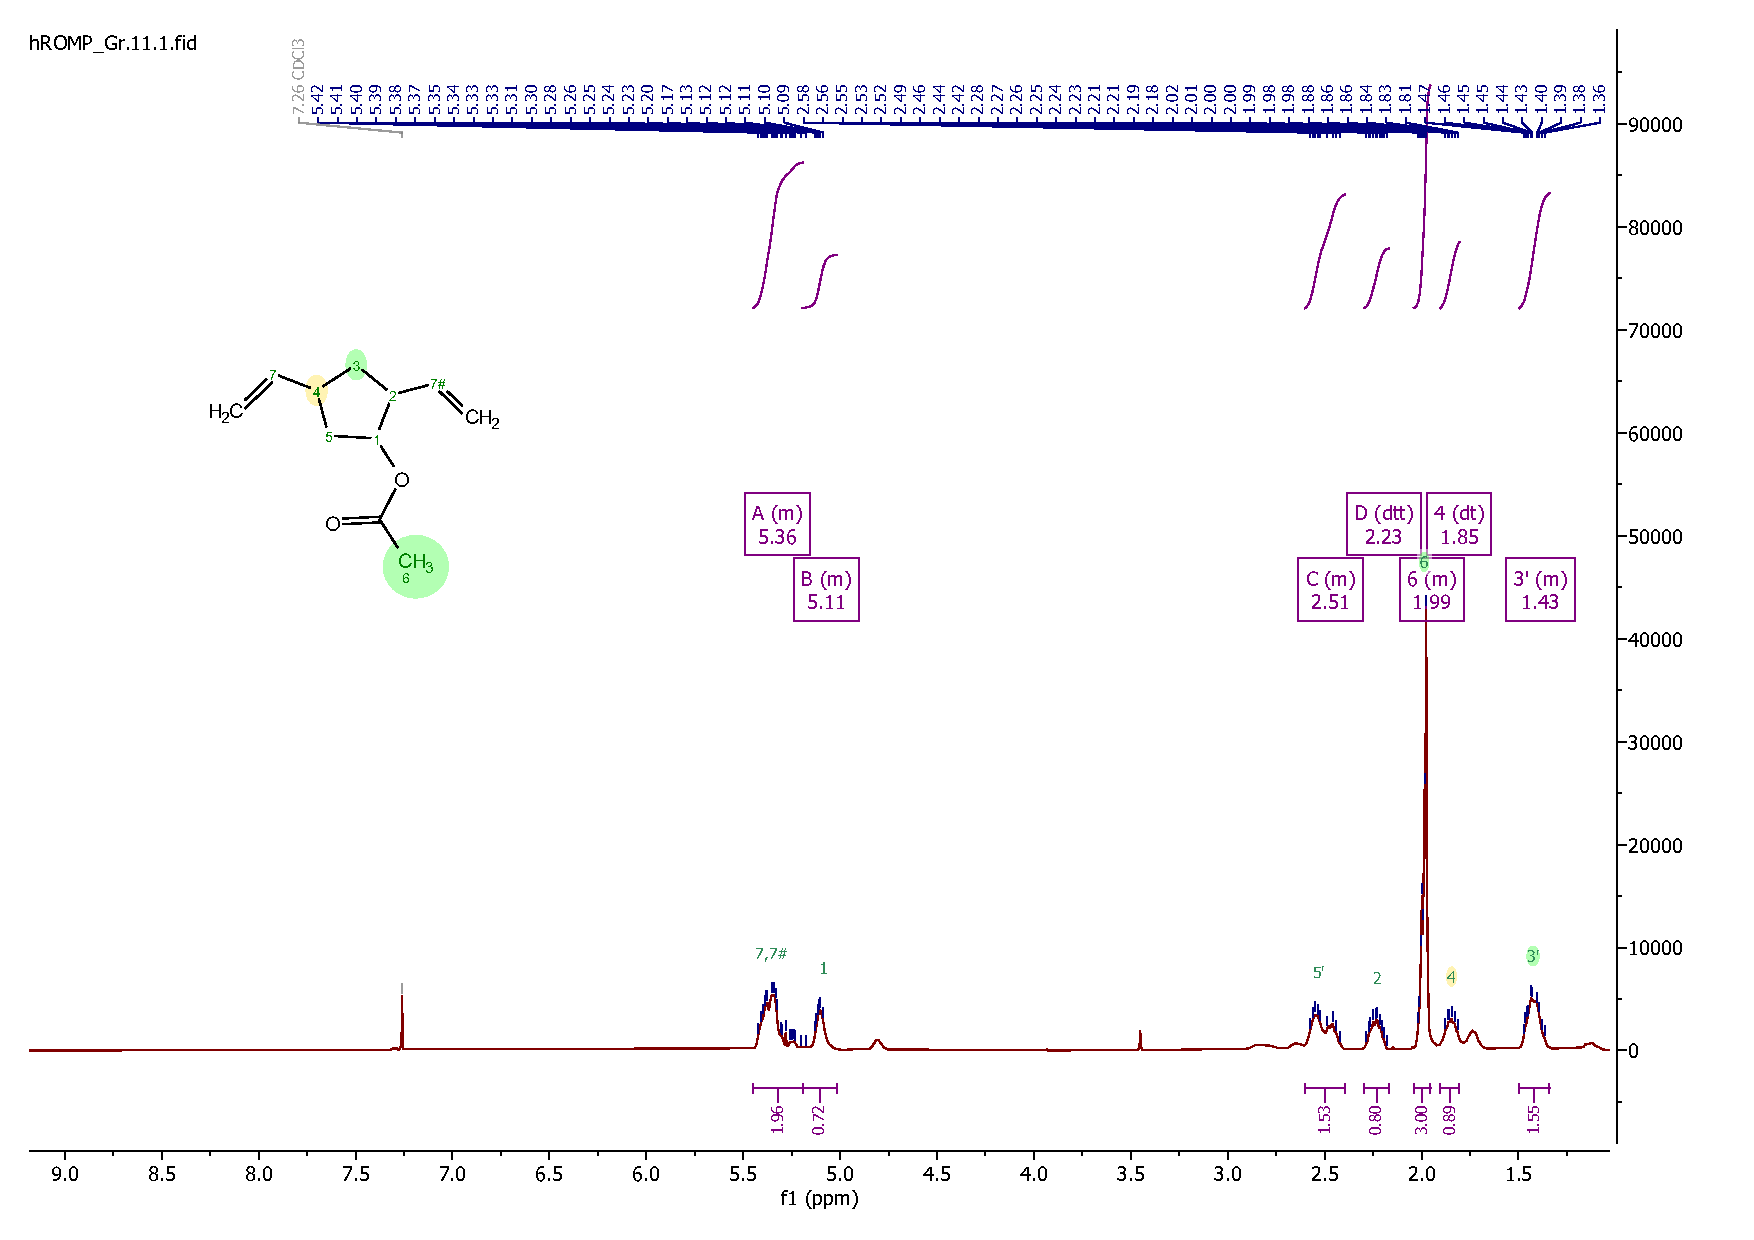
\includegraphics[scale = 0.5]{NMR/hROMP_Gr.11.1.fid.pdf}
					\caption{Die Abbildung zeigt das NMR des Polymers aus Versuchsteil 2.}
					\label{NMR}
				\end{figure}

			Bei genauerem Betrachten des NMR, fällt zunächst der große Peak (E) auf, welcher den drei Wasserstoffen an der Methylgruppe des Esters entspricht.
			Im ähnlichen Bereich kommen die aliphatische Wasserstoffe, welche im Backbone Ring des Polymers sind. 
			Die Peaks im Tieffeld, sind die beiden Wasserstoffe der Kohlenstoffe an der Doppelbindung, diese sind im olephinischen Bereich (Peak A) mit einem passenden Integral von 2.
			Das andere tieffeld verschobene Signal bei 5.11, ist dem Wasserstoff am Kohlenstoff direkt an dem Sauerstoff der Estergruppe zuzuordnen (Peak B) mit einem passenden Integral von 1.


\printbibliography

\end{document}